% Section 7: two routes to the same number for a = (1, 2), b = (3, 1) and the degree-2 kernel.
% Top: build phi(a), phi(b) in 3D, then take their dot product. Bottom: 2D dot product, then square.
\documentclass[tikz,border=8pt]{standalone}
% Shared look for every TikZ diagram. Load with \input{../../tools/tikz-style.tex}
\usepackage[T1]{fontenc}
\usepackage{lmodern}
\renewcommand{\sfdefault}{lmr}  % diagrams use the same serif as the text
\usetikzlibrary{arrows.meta, positioning, shapes.geometric, calc, fit, backgrounds}
\definecolor{cblue}{HTML}{4C78A8}
\definecolor{corange}{HTML}{F58518}
\definecolor{cgreen}{HTML}{54A24B}
\definecolor{cred}{HTML}{E45756}
\definecolor{cpurple}{HTML}{B279A2}
\definecolor{cgrey}{HTML}{6B6B6B}
\tikzset{
  every picture/.style={font=\sffamily, line width=1.2pt},
  box/.style={draw=#1, fill=#1!12, rounded corners=4pt, align=center, inner sep=7pt, minimum height=1.1cm},
  box/.default=cgrey,
  arrow/.style={-{Stealth[length=3mm]}, draw=cgrey, line width=1.4pt},
  title/.style={font=\sffamily\bfseries\Large},
  note/.style={font=\sffamily\small, text=cgrey, align=center},
}
\AtBeginDocument{\hyphenpenalty=10000 \exhyphenpenalty=10000}

\begin{document}
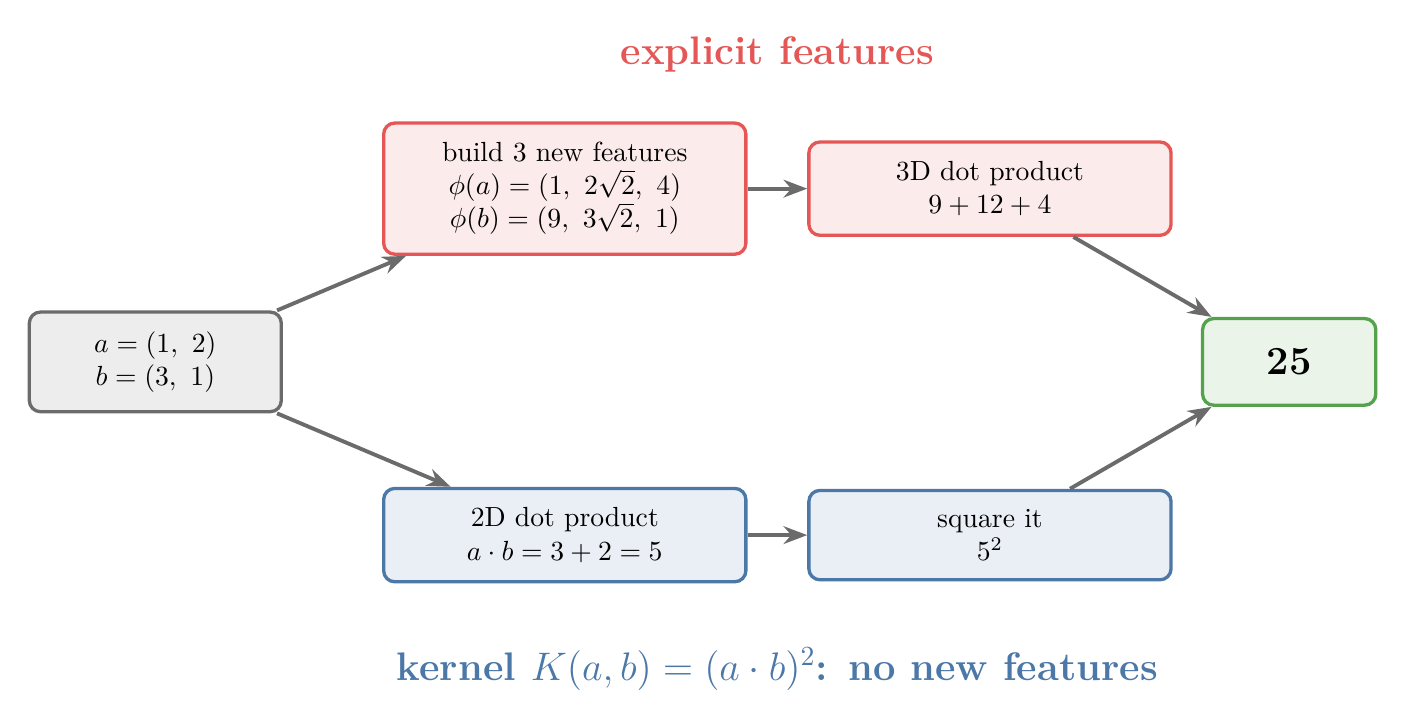
\begin{tikzpicture}[
  d/.style={box=cgrey, minimum width=3.2cm},
  e/.style={box=cred, minimum width=4.6cm},
  k/.style={box=cblue, minimum width=4.6cm},
  r/.style={box=cgreen, minimum width=2.2cm, font=\sffamily\bfseries\Large}]
  \node[d] (in) at (0,0) {$a = (1,\ 2)$\\$b = (3,\ 1)$};
  % explicit route
  \node[e] (phi) at (5.2,2.2) {build 3 new features\\$\phi(a) = (1,\ 2\sqrt{2},\ 4)$\\$\phi(b) = (9,\ 3\sqrt{2},\ 1)$};
  \node[e] (dot3) at (10.6,2.2) {3D dot product\\$9 + 12 + 4$};
  % kernel route
  \node[k] (dot2) at (5.2,-2.2) {2D dot product\\$a \cdot b = 3 + 2 = 5$};
  \node[k] (sq) at (10.6,-2.2) {square it\\$5^2$};
  \node[r] (out) at (14.4,0) {25};
  \draw[arrow] (in) -- (phi); \draw[arrow] (phi) -- (dot3); \draw[arrow] (dot3) -- (out);
  \draw[arrow] (in) -- (dot2); \draw[arrow] (dot2) -- (sq); \draw[arrow] (sq) -- (out);
  \node[title, text=cred] at (7.9,3.9) {explicit features};
  \node[title, text=cblue] at (7.9,-3.9) {kernel $K(a,b) = (a \cdot b)^2$: no new features};
\end{tikzpicture}
\end{document}
